\documentclass[slides]{pgnotes}

\title{Ansible}

\begin{document}

\maketitle

\tableofcontents

\section{Scenario}

\begin{center}
  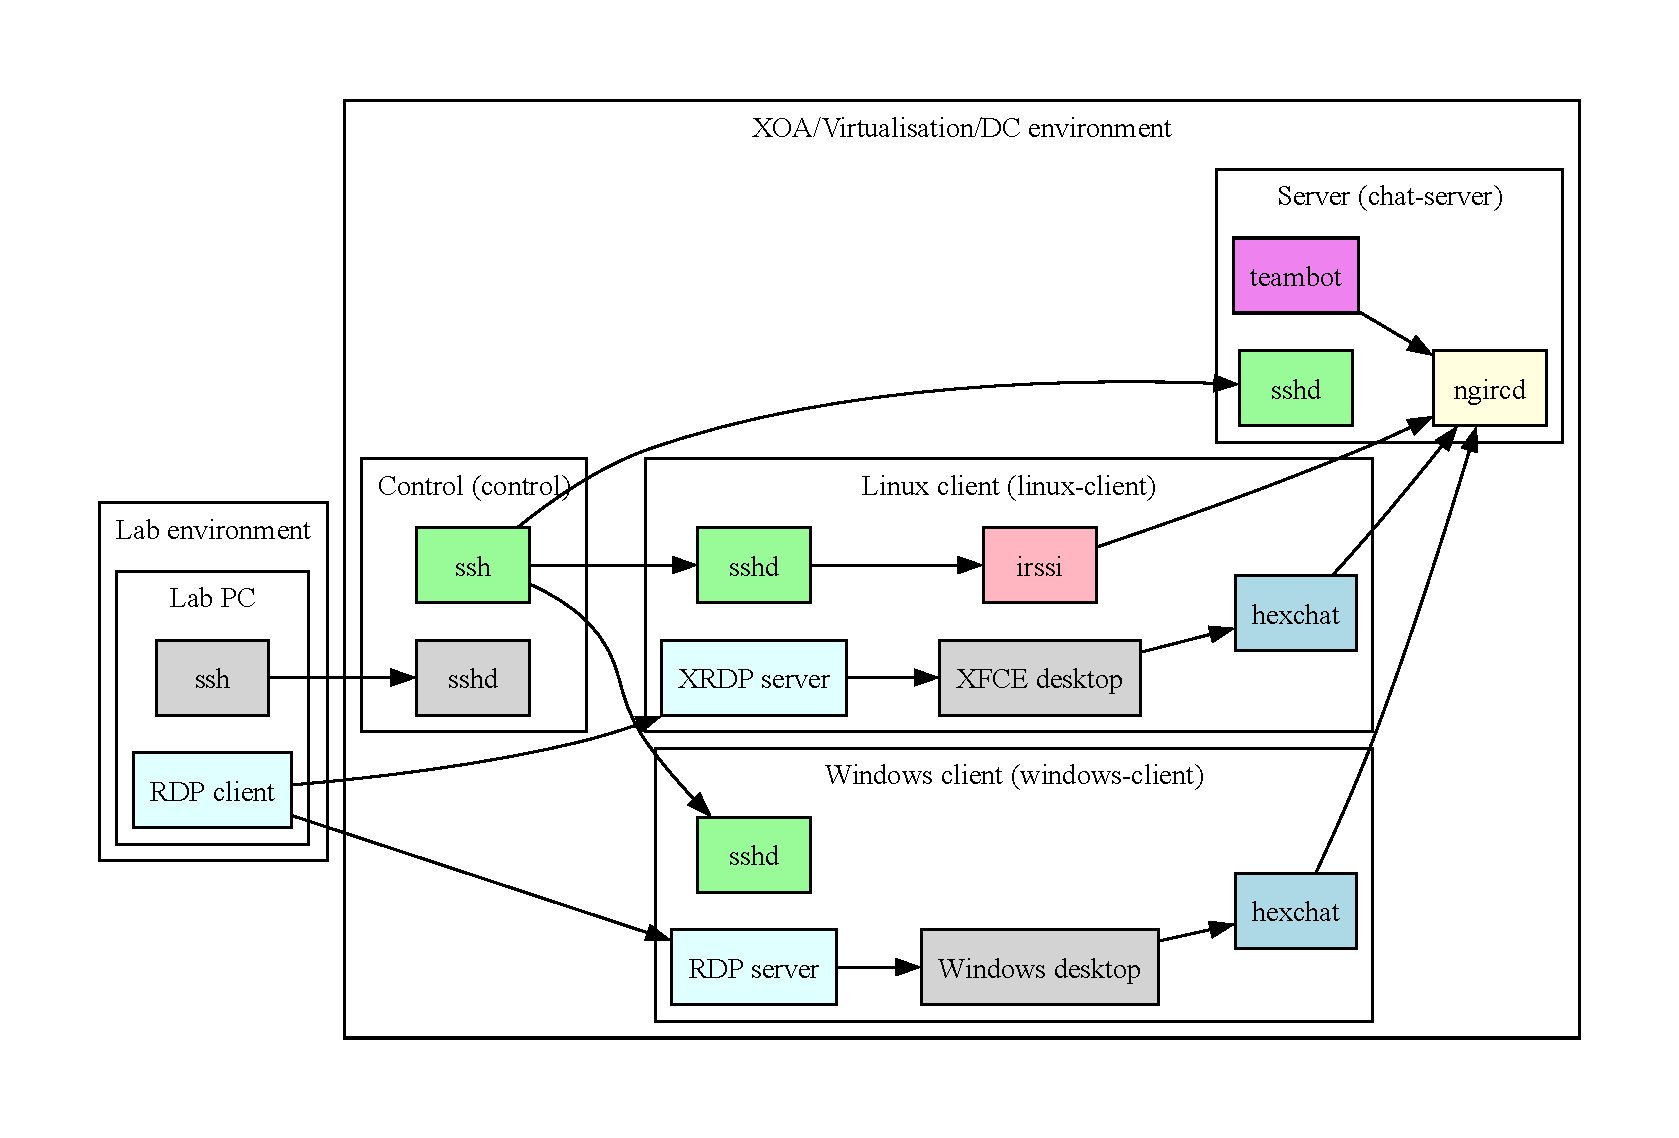
\includegraphics[width=1.0\linewidth]{scenario}
\end{center}


\subsection{Set-up}

\textbf{To save lab time, let's start the set up the 3 machines now (Task 1):}

\section{Components}

\begin{description}
\item[Control node]: System where Ansible is installed.
  \begin{itemize}
  \item You run Ansible commands such as \texttt{ansible} or \texttt{ansible-inventory} on a control node.
  \end{itemize}
  
\item[Inventory]: List of managed nodes that are logically organized.
  \begin{itemize}
  \item Can create inventory on the control node to describe host deployments to Ansible.
  \end{itemize}

\item[Managed node]: Remote system, or host, that Ansible controls.
  \begin{itemize}
  \item May be physical, virtual, cloud VM, SBC like R-Pi etc.
  \end{itemize}

\end{description}

\section{How ansible works}

Ansible is \textbf{agentless}:
\begin{itemize}
\item Some automation solutions require an \textit{agent} to be running on the managed node(s).
\item Ansible uses SSH to let the control node take actions on the managed node.
\item Once you can make an SSH connection from the control to the mangaged node you can run ansible commands on it.
\end{itemize}

\end{document}

